%%%%%%%%%%%%%%%%%%%%%%%%%%%%%%%%%%%%%%%%%
% Beamer Presentation
% LaTeX Template
% Version 1.0 (10/11/12)
%
% This template has been downloaded from:
% http://www.LaTeXTemplates.com
%
% License:
% CC BY-NC-SA 3.0 (http://creativecommons.org/licenses/by-nc-sa/3.0/)
%
%%%%%%%%%%%%%%%%%%%%%%%%%%%%%%%%%%%%%%%%%

 
%----------------------------------------------------------------------------------------
%	PACKAGES AND THEMES
%----------------------------------------------------------------------------------------

\documentclass[15pt]{beamer}
\usepackage[utf8]{inputenc}
\usepackage{amsmath}
\usepackage{graphicx}
\usepackage{hyperref}
\usepackage{float}
\usepackage{wrapfig}
\usepackage{comment} % enables the use of multi-line comments (\ifx \fi) 
\usepackage{lipsum} %This package just generates Lorem Ipsum filler text.
%\usepackage[french]{babel}
\pdfmapfile{+sansmathaccent.map}

\mode<presentation> {

% The Beamer class comes with a number of default slide themes
% which change the colors and layouts of slides. Below this is a list
% of all the themes, uncomment each in turn to see what they look like.

%\usetheme{default}
%\usetheme{AnnArbor}
%\usetheme{Antibes}
%\usetheme{Bergen}
%\usetheme{Berkeley}
%\usetheme{Berlin}
%\usetheme{Boadilla}
%\usetheme{CambridgeUS}
%\usetheme{Copenhagen}
%\usetheme{Darmstadt}
%\usetheme{Dresden}
%\usetheme{Frankfurt}
%\usetheme{Goettingen}
%\usetheme{Hannover}
%\usetheme{Ilmenau}
%\usetheme{JuanLesPins}
%\usetheme{Luebeck}
%\usetheme{Madrid}
%\usetheme{Malmoe}
%\usetheme{Marburg}
\usetheme{Montpellier}
%\usetheme{PaloAlto}
%\usetheme{Pittsburgh}
%\usetheme{Rochester}
%\usetheme{Singapore}
%\usetheme{Szeged}
%\usetheme{Warsaw}

% As well as themes, the Beamer class has a number of color themes
% for any slide theme. Uncomment each of these in turn to see how it
% changes the colors of your current slide theme.

%\usecolortheme{albatross}
\usecolortheme{beaver}
%\usecolortheme{beetle}
%\usecolortheme{crane}
%\usecolortheme{dolphin}
%\usecolortheme{dove}
%\usecolortheme{fly}
%\usecolortheme{lily}
%\usecolortheme{orchid}
%\usecolortheme{rose}
%\usecolortheme{seagull}
%\usecolortheme{seahorse}
%\usecolortheme{whale}
%\usecolortheme{wolverine}

%\setbeamertemplate{footline} % To remove the footer line in all slides uncomment this line
\setbeamertemplate{footline}[page number] % To replace the footer line in all slides with a simple slide count uncomment this line

%\setbeamertemplate{navigation symbols}{} % To remove the navigation symbols from the bottom of all slides uncomment this line
}

\usepackage{graphicx} % Allows including images
\usepackage{booktabs} % Allows the use of \toprule, \midrule and \bottomrule in tables

%----------------------------------------------------------------------------------------
%	TITLE PAGE
%----------------------------------------------------------------------------------------

\title{Multilayer and stream graphs} % The short title appears at the bottom of every slide, the full title is only on the title page

\author{Pimprenelle Parmentier} % Your name



\date{\today} % Date, can be changed to a custom date



\begin{document}

\begin{frame}
\titlepage % Print the title page as the first slide
\end{frame}

%\begin{frame}
%\frametitle{Plan} % Table of contents slide, comment this block out to remove it
%\tableofcontents % Throughout your presentation, if you choose to use \section{} and \subsection{} commands, these will automatically be printed on this slide as an overview of your presentation
%\end{frame}

%----------------------------------------------------------------------------------------
%	PRESENTATION SLIDES
%----------------------------------------------------------------------------------------

%------------------------------------------------

\section{Introduction} % Sections can be created in order to organize your presentation into discrete blocks, all sections and subsections are automatically printed in the table of contents as an overview of the talk

\begin{frame}{The basic notions}
\begin{minipage}[t]{5cm}
\textbf{Multilayer graphs}
\\
$M=(V_M,E_M,V,L)$
\\
\begin{itemize}
    \item Different types of interaction
    \item Different types of nodes
    \item More complex structures
\end{itemize}
\begin{figure}
    \centering
    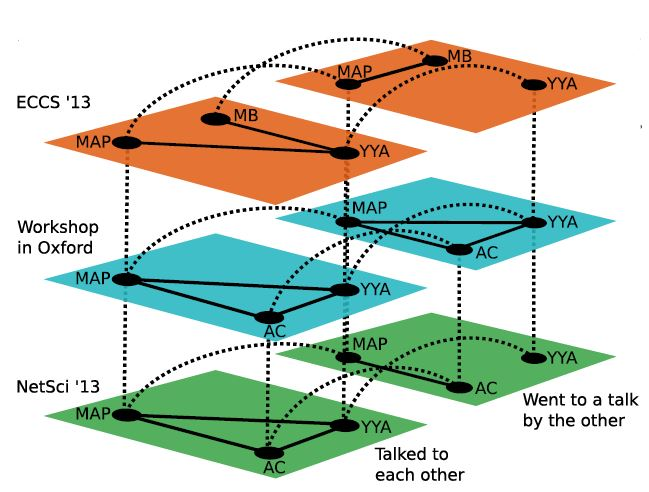
\includegraphics[width=4cm]{img/exMulti.JPG}
    \label{fig:exmulti}
\end{figure}
\end{minipage}
\begin{minipage}[t]{5cm}
\textbf{Stream Graphs}
\\
$S=(T,V,W,E)$
\begin{itemize}
    \item nodes can appear or desappear in function of continuous time
    \item links can appear or desappear in function of continuous time
\end{itemize}
\begin{figure}
    \centering
    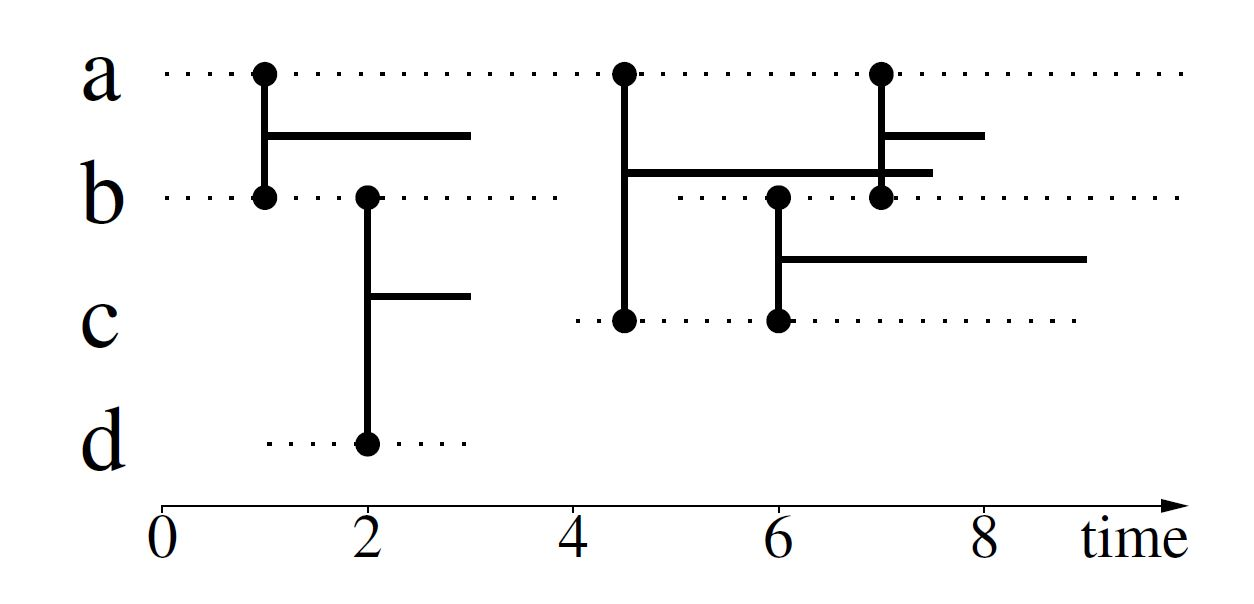
\includegraphics[width=4cm]{img/exampleStream.JPG}
    \label{fig:exstream}
\end{figure}
\end{minipage}

\end{frame}

\begin{frame}{The multilayer stream graph}
\[
G=(T,T_M,V,W_M,E_M,\cal{L})
\]
%\begin{minipage}{10cm}
%\begin{itemize}
%	\item nodes and links can appear at different times in different layers
%	\item layers can appear and disappear at different times
%\end{itemize}
%\end{minipage}

\begin{figure}
    \centering
    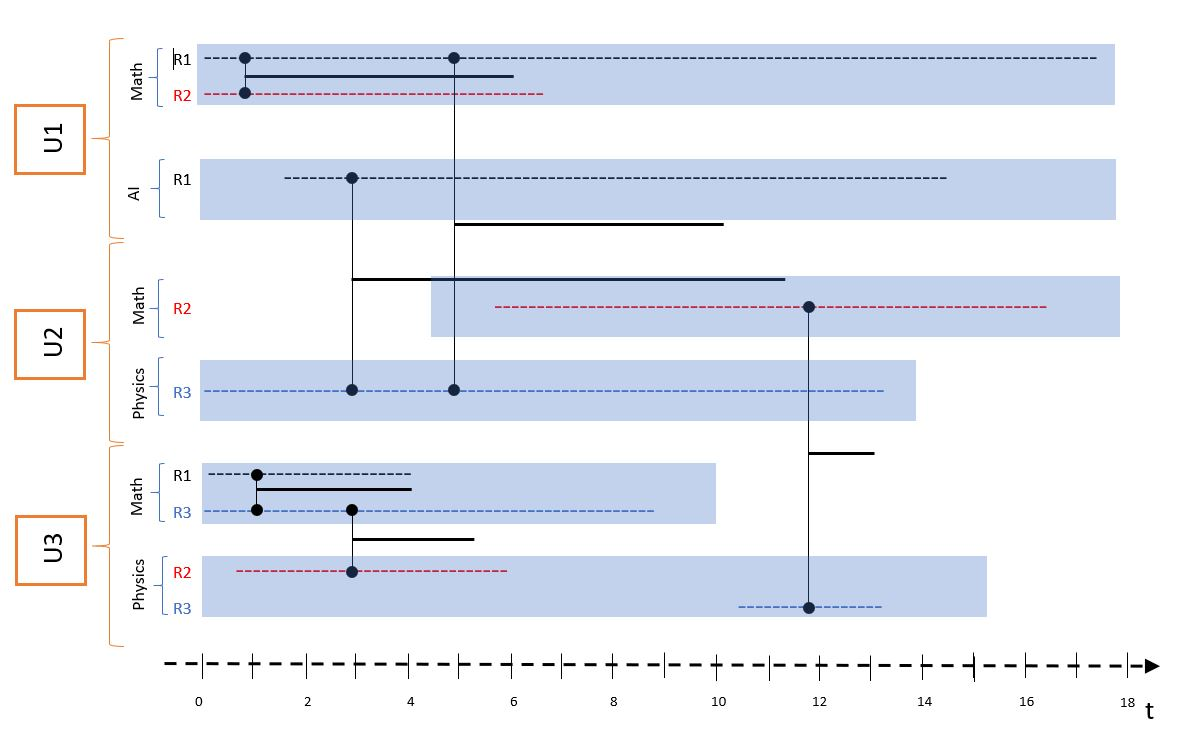
\includegraphics[width=8cm]{img/chercheurs.jpg}
    \label{fig:chercheurs}
\end{figure}
\end{frame}

\begin{frame}{Application areas}
A good dataset should have :
\begin{itemize}
    \item time-dependence
    \item different types of nodes and/or different types of links
\end{itemize}
A few examples :
\begin{itemize}
    \item social interactions
    \item biological interactions
    \item information network
    \item transportation network
    \item diffusion (epidemics, etc)
\end{itemize}
\end{frame}
\begin{frame}{Our goals...}

What we want to do : 
\begin{itemize}
    \item find the "decisive" times and and nodes/links/layer : stop a diffusion, find a weakness in the network...
    \item measure "influence" : find a "precursor", find which parameter are "important" and which are not (ex : most of researchers in dept D in university U at time T became "influent") ...
    \item measure "intrication" : how much a group of layers are "superimposed" (ex: the relationships of type "co-workers in this company" are "strongly correlated" to most of the overall relationships)
    \item determinate if two multilayer-streams have the same structure (isomorphism)
\end{itemize}
    
\end{frame}

\begin{frame}{Let's talk and brainstorm...}
    Questions ?
    \\
    Ideas ? Suggestions ?
\end{frame}
\end{document}